\documentclass[11pt]{article}

\usepackage[a4paper,margin=1.05in]{geometry}
\usepackage[T1]{fontenc}
\usepackage{lmodern}
\usepackage{microtype}
\usepackage{amsmath,amssymb,amsthm}
\usepackage{booktabs}
\usepackage{graphicx}
\usepackage{caption}
\usepackage{threeparttable}
\usepackage{setspace}
\usepackage[round]{natbib}
\usepackage{xurl}
\usepackage[
  colorlinks=true,
  linkcolor=blue,
  citecolor=blue,
  urlcolor=blue
]{hyperref}

\captionsetup{font=small,labelfont=bf,skip=6pt}
\setstretch{1.12}
\setlength{\parskip}{0.25em}
\setlength{\emergencystretch}{1.5em}

\newtheorem{proposition}{Proposition}
\newtheorem{lemma}{Lemma}
\newtheorem{corollary}{Corollary}
\theoremstyle{definition}
\newtheorem{assumption}{Assumption}
\theoremstyle{remark}
\newtheorem{remark}{Remark}

\makeatletter
% expandable file input for table rows inside tabular environments
\newcommand{\tablerows}[1]{\@@input#1 }
\makeatother

\newcommand{\E}{\mathbb{E}}
\newcommand{\R}{\mathbb{R}}
\newcommand{\lgt}{\operatorname{logit}}
\newcommand{\D}{\mathcal{D}}
\newcommand{\K}{\mathcal{K}}

\newcommand{\Rho}{0.864}
\newcommand{\RhoSE}{0.054}
\newcommand{\RhoBC}{0.985}
\newcommand{\HalfLife}{4.7}
\newcommand{\StateN}{2090}
\newcommand{\StateCountries}{135}
\newcommand{\NetworkSlope}{1.049}
\newcommand{\BootReps}{399}
\newcommand{\GrowthOne}{-1.48}
\newcommand{\FragilityOne}{-0.45}
\newcommand{\GrowthTwo}{-1.52}
\newcommand{\FragilityTwo}{-0.94}
\newcommand{\GrowthThree}{-1.40}
\newcommand{\FragilityThree}{-1.35}
\newcommand{\QuantileTen}{-0.71}
\newcommand{\QuantileTwentyFive}{-0.61}
\newcommand{\QuantileFifty}{-0.55}
\newcommand{\QuantileSeventyFive}{-0.65}
\newcommand{\QuantileNinety}{-0.82}
\newcommand{\ForecastTail}{-3.22}
\newcommand{\ForecastMedian}{-0.41}
\newcommand{\ForecastUpper}{-2.30}
\newcommand{\ForecastMean}{-0.14}


\begin{document}

\hypersetup{pageanchor=false}
\begin{titlepage}
\begin{center}
\vspace*{1cm}

{\LARGE Disinformation, Financial Fragility,
and Downside Growth Risk\par}

\vspace{1cm}

{\large James Rice\footnote{Policy Fellow, Council for Countering Online
Disinformation. Email: \texttt{ricejames0@gmail.com}. I thank colleagues at
the Council for Countering Online Disinformation for comments on the research
proposal that preceded this paper. Selected algebraic results have companion Lean~4 formalizations
against mathlib \citep{moura2021lean,mathlib2020lean}; the replication
appendix specifies their scope. They do not verify empirical identification
or policy effectiveness. All remaining errors are my own.}\par}


{\normalsize September 2026\par}



\begin{abstract}
\noindent
This paper examines whether a broad disinformation index is associated
with downside growth risk and financial fragility. A panel of 175 countries
from 2000 to 2025 combines expert-coded Digital Society Project indicators
with macroeconomic outcomes. The index measures the political information
environment, not the prevalence of false financial messages. Panel local
projections estimate a three-year cumulative-growth association of
$\GrowthTwo$ percentage points per standard deviation of the index at mean
conditioning states. The banking-stress interaction is $\FragilityTwo$.
Country-block bootstrap contrasts do not distinguish the lower-tail
slope from the median or upper tail. A chronological forecast comparison
provides no evidence of improved downside prediction in the evaluated design. The tenth-quantile forecast-loss gain from adding the index is
$\ForecastTail$ percent; negative gains indicate worse performance.
An illustrative financing model gives increasing differences in contamination
and fragility. Aggregate index persistence is distinct from individual
narrative lifetimes, and a half-life elasticity comparison ranks parameter
changes only under explicit sign, cost and effectiveness assumptions.
The evidence is observational and does not identify financial-message harm,
a crisis threshold or causal returns to information policy.
\end{abstract}
\end{center}
{\small\raggedright \textbf{JEL codes:} D83, D84, E32, E44, G01, G28, L86.\\
\textbf{Keywords:} disinformation, information pollution, narrative
economics, growth-at-risk, financial fragility, local
projections.\par}
\end{titlepage}
\hypersetup{pageanchor=true}

\section{Introduction}\label{sec:intro}

Misleading information can affect financial decisions through attention,
beliefs and confidence. Evidence on manipulated financial news and social
media during bank runs establishes the relevance of information transmission
for financial markets \citep{kogan2023social,clarke2021fake,cookson2023social}.
Social-media amplification is not itself evidence that the amplified claims
were false. A distinct macroeconomic question is whether an information
environment characterized by frequent disinformation is associated with worse
growth outcomes, particularly when financial conditions are fragile.

This paper investigates that question with a country panel and an
illustrative financing mechanism. Its empirical contribution is a transparent
assessment of the information content of a broad disinformation proxy,
including conditional mean associations, quantile slopes, fragility
interactions and chronological forecast evaluation. It does not estimate
the causal macroeconomic effect of financial misinformation or the returns
to a particular content intervention.

The mechanism combines signal contamination with an explicitly assumed
noise-sensitive lending rule. The resulting investment shortfall has
increasing differences in contamination and fragility: deterioration in
information can matter more when financing constraints are close to binding.
A separate feedback example permits multiple steady states. A scalar
persistence calculation gives a conditional comparison of equal proportional
changes in model parameters. These results clarify hypotheses and identify
assumptions needed for policy analysis; they are not substitutes for
measurement or identification.

The empirical proxy combines five DSP indicators of government and party
disinformation in 175 countries over 2000--2025. It measures relative intensity
in the political information environment, rather than the share of financial
messages that are false. The analysis retains that distinction
throughout. The local projections estimate associations with cumulative
outcomes, while separate quantile regressions assess whether slopes differ
across the conditional growth distribution. Financial stress is a
conditioning state, not an externally assigned treatment.

The three-year cumulative-growth coefficient is
$\GrowthTwo$ percentage points per standard deviation of the index at mean
conditioning states. The corresponding banking-stress interaction is
$\FragilityTwo$ points. Two-year conditional growth slopes are
$\QuantileTen$, $\QuantileFifty$ and $\QuantileNinety$ points at the tenth,
fiftieth and ninetieth percentiles. These numbers must be evaluated with their
uncertainty, sample variation and reverse-timing diagnostics, rather than
interpreted as treatment effects. Joint bootstrap comparisons do not distinguish the lower-tail slope
from the median or upper tail, so the data do not support a
disproportionately large downside association.

The forecasting extension compares the same macro-financial benchmark with
and without the index. It fits component scaling and ranks solely within
each training window and respects a one-year predictor-availability lag.
Across held-out target years 2015--2024, the change in tenth-quantile pinball
loss is reported as a $\ForecastTail$ percent gain, where negative values
mean worse performance. The evaluated design does not support improved downside-risk
prediction from adding the index. Latest-vintage source data and a
short evaluation period remain material limitations.

\paragraph{Related literature.}
Models of misinformation and narrative formation study platform incentives,
social learning and competing explanations
\citep{acemoglu2024model,muellerfrank2024weakest,eliaz2020model}.
Experimental work documents motivated evaluation and incomplete updating after
retractions \citep{thaler2024fake,goncalves2026retractions}. Evidence on
political misperceptions and institutional confidence reinforces the need to
distinguish a political-information proxy from financial-content exposure
\citep{cariolle2024misinformation,guriev20213g,zhuravskaya2020political}.
Assessments of misinformation also warn against extrapolating from vivid
incidents to aggregate harm \citep{budak2024misunderstanding,altay2023misinformation}.

The macroeconomic motivation comes from narrative economics
\citep{shiller2017narrative,shiller2019narrative}, vulnerable-growth methods
\citep{adrian2019vulnerable}, and collateral-based amplification
\citep{kiyotaki1997credit,bernanke1999financial}. The feedback illustration
is related to uncertainty traps \citep{fajgelbaum2017uncertainty}.
The empirical tools are local projections \citep{jorda2005estimation} and
two-step panel quantile estimation \citep{canay2011simple}. Applying those
tools to a persistent observational index does not by itself identify a
structural shock. The paper's contribution lies in the combination of
measurement discipline, reproducible conditional evidence, and explicit
predictive validation.

Section~\ref{sec:model} develops the illustrative mechanism;
Section~\ref{sec:data} explains measurement; Section~\ref{sec:empirics}
presents estimation and validation. Sections~\ref{sec:risk} and
\ref{sec:policy} delimit risk and policy interpretations, and
Section~\ref{sec:conclusion} concludes. The appendix provides proofs,
robustness results and replication details.

\section{An Illustrative Mechanism and Its Limits}\label{sec:model}

The model separates an observed proxy for the information environment from
financial-message contamination. Its role is to organize hypotheses about
conditional associations. The country panel does not identify its structural
parameters or a causal response to information policy.

\subsection{A bounded information-environment proxy}\label{subsec:state}
Let $M_t\in(0,1)$ denote a normalized information-environment index and
$x_t=\lgt(M_t)$. Consider
\begin{equation}\label{eq:state}
 x_{t+1}=c+\rho x_t+\delta s_t+u_{t+1}.
\end{equation}
Here $c$ is an intercept in logit units, $\rho$ is conditional persistence,
and $s_t$ summarizes other countries' index values. An intercept can be
negative; it is not a count or physical inflow of false messages. The
observed index is a rank, so neither $M_t$ nor $x_t$ measures the share of
financial claims that are false. The process offers a parsimonious description
of persistence in an information environment, motivated by narrative economics
\citep{shiller2017narrative,shiller2019narrative}.

\begin{proposition}[Scalar dynamics conditional on external inputs]\label{prop:state}
With $s_t=0$, $u_t=0$ and $0<\rho<1$, the unique steady state is
$\mu=c/(1-\rho)$, and
$x_t=\mu+\rho^t(x_0-\mu)$. Consequently $M_t=\sigma(x_t)\in(0,1)$ and
converges to $\sigma(\mu)$. With independent mean-zero innovations of
variance $\sigma_u^2$, the stationary latent variance is
$\sigma_u^2/(1-\rho^2)$. A deviation in the latent state has half-life
$h_{1/2}=\ln(2)/[-\ln(\rho)]$, exceeding one observation period precisely
when $\rho>1/2$.
\end{proposition}

This half-life concerns a deviation of the aggregate latent index, not the
survival time of a particular narrative. In the stochastic model,
$\E[\sigma(x)]$ generally differs from $\sigma(\E[x])$. The nonlinear
index also need not inherit the latent state's exact half-life.
For jointly evolving countries with a fixed row-stochastic regional matrix
$W$, the corresponding linear system is
$x_{t+1}=c+(\rho I+\delta W)x_t+u_{t+1}$. Its stability requires the
spectral radius of $\rho I+\delta W$ to be below one. For nonnegative
$\rho,\delta$, that radius equals $\rho+\delta$. Scalar stability alone
therefore does not establish stability of an endogenous regional system.

The distinction between latent and observed persistence can be made explicit.
For a deterministic initial deviation $d_0=x_0-\mu$, the observed deviation is
\begin{equation}\label{eq:index-deviation}
 M_t-\sigma(\mu)=\sigma(\mu+\rho^td_0)-\sigma(\mu).
\end{equation}
Because $0<\sigma'(x)=\sigma(x)\{1-\sigma(x)\}\le1/4$, its absolute
value is at most $\rho^t|d_0|/4$. Close to the steady state it is approximately
$\sigma'(\mu)\rho^td_0$. Thus a common latent persistence can coexist with
different movements in the bounded index: the same latent deviation produces
a smaller index change near either endpoint than near its midpoint. Ranking
countries before taking logits further makes this a statement about relative
information environments, rather than absolute quantities of false content.

Persistence also makes long-run summaries sensitive to estimation error.
Writing $h(\rho)=\log(2)/[-\log(\rho)]$ gives
\begin{equation}\label{eq:half-sensitivity}
 h'(\rho)=\frac{\log(2)}{\rho\{\log(\rho)\}^2}>0,
 \qquad h(\rho)\sim\frac{\log(2)}{1-\rho}\quad\text{as }\rho\uparrow1.
\end{equation}
The half-life therefore becomes highly sensitive near unity. This explains
why the baseline persistence $\Rho$ implies $\HalfLife$ years whereas the
approximation $\RhoBC$ implies a much longer horizon. Transforming a point
estimate is useful for interpretation, but it does not remove uncertainty in
the estimated dynamics. An interval reaching unity cannot be mapped into a
finite upper bound on a stationary half-life.

\subsection{Contamination and financing constraints}\label{subsec:pollution}
Let $p\in[0,1]$ be the unobserved probability that a financial signal is
contaminated. A signal about collateral value $V$ is
$s=V+b\eta d+\varepsilon$, where $b\sim\mathrm{Bernoulli}(p)$,
$\eta\in\{-1,1\}$ has equal probabilities, $d>0$, and $\varepsilon$ has
mean zero and variance $\sigma_\varepsilon^2$. Assume the disturbances and
$V$ are mutually independent, conditional on $p$.

\begin{lemma}[Signal contamination]\label{lem:pollution}
$\E[s\mid V,p]=V$ and
$\mathrm{Var}(s\mid V,p)=\sigma_\varepsilon^2+pd^2$.
\end{lemma}

The lemma is about signal noise conditional on the fundamental. It is not a
formula for posterior uncertainty $\mathrm{Var}(V\mid s,p)$, which also
depends on the prior and the signal likelihood. To obtain a transparent
financing mechanism, assume directly that lenders apply a haircut increasing
in noise variance:
\begin{equation}\label{eq:credit}
 L(p)=\lambda\{\bar V-\gamma(\sigma_\varepsilon^2+pd^2)\},
 \qquad \lambda,\gamma\ge0.
\end{equation}
Restrict attention to $L(p)\ge0$; this is a reduced-form credit rule rather
than a derived Bayesian valuation. An entrepreneur with net worth $W_0$ and
desired investment $I^*$ invests $\min\{I^*,W_0+L(p)\}$. The resulting
shortfall can be written
\begin{equation}\label{eq:harm}
 H(p,F)=\max\{ap+bF-\kappa_0,0\},\qquad a,b\ge0,
\end{equation}
where $a=\lambda\gamma d^2$ and $F$ summarizes financing pressure. This
illustration connects noisy information and collateral constraints
\citep{kiyotaki1997credit,bernanke1999financial,bond2012real}.

\begin{proposition}[Increasing differences]\label{prop:amplification}
For $p_1\le p_2$ and $F_1\le F_2$,
$H(p_2,F_1)-H(p_1,F_1)\le H(p_2,F_2)-H(p_1,F_2)$.
If $ap_2+bF-\kappa_0\le0$, the incremental shortfall is zero.
\end{proposition}

Linking this mechanism to the data requires an additional hypothesis that
financial contamination $p$ increases with the broad index $M$, conditional
on other determinants. This mapping is neither observed nor estimated.
Increasing differences survive a monotone mapping $p(M)$, but the magnitude
and a linear interaction specification do not follow from ranks alone.
Moreover, Proposition~\ref{prop:amplification} does not establish small mean
effects or an ordering of growth-quantile slopes without assumptions about
how fragility, constraints and other shocks populate the outcome distribution.
Those patterns are empirical questions, not consequences of the proposition
by themselves.

\subsection{Aggregation and the meaning of a stress interaction}\label{subsec:aggregation}
Heterogeneity in financing slack connects the individual constraint to a
smooth aggregate relationship. Let $K$ be an entrepreneur's slack threshold,
with distribution function $C_K$ and continuous density $f_K$. Hold this
distribution fixed as $p$ and $F$ vary, assume $\E|K|<\infty$, and let $a,b$
be common nonnegative coefficients. Average shortfall is
\begin{equation}\label{eq:aggregate-harm}
 \overline H(p,F)=\E_K[(ap+bF-K)_+],\qquad (z)_+=\max\{z,0\}.
\end{equation}
The fixed-distribution assumption isolates the constraint mechanism;
selection into borrowing or changing firm composition can create additional
effects that are not represented here.

\begin{proposition}[Aggregate constraint exposure]\label{prop:aggregation}
Under these assumptions,
\begin{equation}\label{eq:aggregate-derivatives}
 \overline H_p=aC_K(ap+bF),\qquad
 \overline H_{pF}=ab f_K(ap+bF)\ge0.
\end{equation}
If growth obeys $y=y^0-\chi\overline H(p,F)+\epsilon$ with $\chi\ge0$,
and $p=p(m)$ is differentiable and nondecreasing in an index coordinate $m$,
then, holding $y^0$ and the distribution of $\epsilon$ fixed,
\begin{equation}\label{eq:growth-cross}
 \frac{\partial y}{\partial m}
 =-\chi a p'(m)C_K(ap(m)+bF),\qquad
 \frac{\partial^2 y}{\partial m\,\partial F}
 =-\chi ab p'(m)f_K(ap(m)+bF)\le0.
\end{equation}
\end{proposition}

The level slope depends on the fraction already constrained. The interaction
depends on the density close to the constraint boundary: a rise in fragility
moves additional entrepreneurs into the region where information noise
restricts investment. If almost nobody is constrained, the level association
can be small. If almost everybody is constrained, shortfall can be large but
its interaction with further stress can be small. Strong amplification is
therefore most plausible where an appreciable mass lies near the boundary.

A local expansion around reference values $(m_0,F_0)$ contains
$y_m(m-m_0)$ and $y_{mF}(m-m_0)(F-F_0)$, alongside linear stress and
own-variable curvature terms. The empirical interaction is a tractable
approximation to this surface. Its magnitude combines the prevalence and
density of constraints, the credit sensitivity $a$, growth conversion $\chi$,
the unobserved mapping $p'(m)$ and the units of both regressors. The panel's
linear projection also averages over heterogeneous observations and need not
equal a structural derivative at a particular point. Consequently the
negative interaction $\FragilityTwo$ is consistent with the mechanism's sign
restriction but cannot separately estimate any of these structural objects.

\paragraph{Why amplification need not imply a steeper lower tail.}
Consider the additional location-scale specification
\begin{equation}\label{eq:location-scale}
 y=\ell(m,F)+s(m,F)\epsilon,\qquad s(m,F)>0,
 \qquad Q_\tau(y\mid m,F)=\ell(m,F)+s(m,F)q_\tau,
\end{equation}
where $\epsilon$ has a fixed continuous distribution independent of $(m,F)$
and $q_\tau$ is its $\tau$ quantile. A financing shortfall may enter
$\ell$ through $-\chi\overline H$ without changing $s$. In that case the
index shifts every conditional quantile by the same amount even if
$\ell_{mF}<0$. More generally, the index-slope difference between two
quantiles is $s_m(q_\tau-q_\nu)$. With $\tau<\nu$, a more negative
lower-tail slope follows from $s_m>0$, an extra dispersion assumption that
increasing differences alone does not supply. The bootstrap contrasts test
whether slopes differ in the fitted quantile specification. Their failure to
distinguish the tails from the median can coexist with a negative
mean-growth interaction with banking stress. This location-scale example
clarifies the distinction without imposing it on the estimated regressions.

\subsection{Feedback as a theoretical possibility}\label{subsec:trap}
Suppose a bounded, increasing function $g:\R\to\R$ describes stress feedback
in latent-state units. Consider
\begin{equation}\label{eq:feedback}
 \psi(x)=c+\rho x+\varphi g(x),\qquad \varphi\ge0.
\end{equation}
Writing $g=G\circ\sigma$ is permissible, but the Lipschitz constant below
is that of the complete composite function on the latent scale.

\begin{proposition}[Uniqueness and possible multiplicity]\label{prop:trap}
If $g$ is globally Lipschitz with constant $L_g$ and
$0\le\rho+\varphi L_g<1$, $\psi$ has a unique globally attracting fixed
point. Multiplicity is possible outside that sufficient condition: with
$c=-3/4$, $\rho=1/2$, $\varphi=2$ and
$g(x)=\min\{\max\{x,0\},1\}$, the fixed points are $-3/2$, $1/2$ and
$5/2$, with stable outer points and an unstable middle point.
\end{proposition}

\begin{samepage}
Failure of the contraction inequality does not prove a bifurcation. A smooth
fold additionally requires a fixed point satisfying $\psi'(x)=1$, with
suitable curvature and transversality conditions. The panel identifies
neither $\varphi$ nor $g$, so the example establishes possibility without
locating countries relative to an escalation threshold.

\subsection{A conditional half-life comparison}\label{subsec:burden}
\begin{proposition}[Comparative statics of the scalar latent steady state]
\label{prop:burden}
For $c>0$ and $0<\rho<1$, the elasticities of
$\mu=c/(1-\rho)>0$ are $\varepsilon_c=1$ and
$\varepsilon_\rho=\rho/(1-\rho)$. Equal infinitesimal proportional reductions
in $\rho$ and $c$ reduce $\mu$ by more under a reduction in persistence precisely when
$\rho>1/2$. For $c\ge0$, $\mu$ is convex in $\rho<1$.
\end{proposition}
\end{samepage}

The common derivative of the logistic transformation cancels when comparing
the two marginal reductions in the deterministic index $\sigma(\mu)$ at
the same baseline. This does not imply the same ranking for stochastic
welfare or a multi-channel burden score. For $c=0$ the proportional elasticity
of $\mu$ is undefined. For $c<0$, reducing $\rho$ raises $\mu$ toward zero
and raises $M$ toward $1/2$; a universal pollution-reduction claim is false.
The observation period must also be fixed: an annual coefficient cannot be
used to rank interventions acting on daily narrative lifetimes.

Let $\eta_\rho=-d\log\rho/dB_\rho$ and
$\eta_c=-d\log c/dB_c$ denote proportional parameter changes per unit of
expenditure, evaluated at positive $c,\rho$. Persistence intervention has the
larger marginal effect on the latent steady state only if
\begin{equation}\label{eq:cost}
 \eta_\rho\frac{\rho}{1-\rho}>\eta_c.
\end{equation}
Equal proportional parameter changes are thus an equal-cost comparison only
when $\eta_\rho=\eta_c$. Neither effectiveness schedule is identified by
the country panel. Corrections, friction and authentication can affect more
than one parameter, further limiting a one-to-one policy interpretation.

\section{Data and Measurement}\label{sec:data}

The starting panel is the repository's frozen merge of the Digital Society
Project (DSP) v8, World Development Indicators (WDI), and Worldwide Governance
Indicators (WGI). It contains 4,539 country-years for 175 countries in
2000--2025. DSP v8 itself covers 179 countries over those years
\citep{mechkova2026dsp}; this coverage does not imply that every regression
contains 175 countries. Observed outcomes and horizon-specific sample sizes
are reported below and in the generated tables.

\subsection{What the index measures}\label{subsec:index}
DSP combines expert assessments through a measurement model
\citep{pemstein2018latent}. The five components concern false-information
dissemination by governments domestically and abroad, political parties
domestically and abroad, and foreign governments into the country. Each
component is reversed so that higher values indicate more disinformation,
then standardized. Weights are respectively $(1/4,1/8,1/4,1/8,1/4)$ in that
ordering. The weighted composite is transformed into its pooled percentile,
using $(\mathrm{rank}-1/2)/n$ with average ranks for ties. The resulting
$M_{r,t}$ lies strictly between zero and one.

These are indicators of the broad political information environment. They
are not financial-content counts, measured exposure, belief adoption or
financial-message accuracy. A value of $0.89$ means approximately the 89th
percentile of the reference distribution; it does not mean that 89 percent
of financial messages are false. No financial-specific validation sample is
available in this replication package. Domestic-only or equal weights probe
index construction but cannot supply that missing construct validity.
The haircut mechanism in Section~\ref{sec:model} therefore motivates a
hypothesis rather than a measured channel.

The retrospective regressions retain the pooled transformation for
comparability. Raw-composite and alternative-weight estimates are reported,
rather than assuming that slopes are invariant to monotone transformations.
For forecasting, component means, standard deviations and the empirical CDF
are re-estimated using each training window only. Evaluation observations
outside the training range are clipped to its finite endpoint ranks. The
DSP component data required for this procedure are included in the
replication data, with source and checksum records.

\begin{figure}[!htbp]\centering
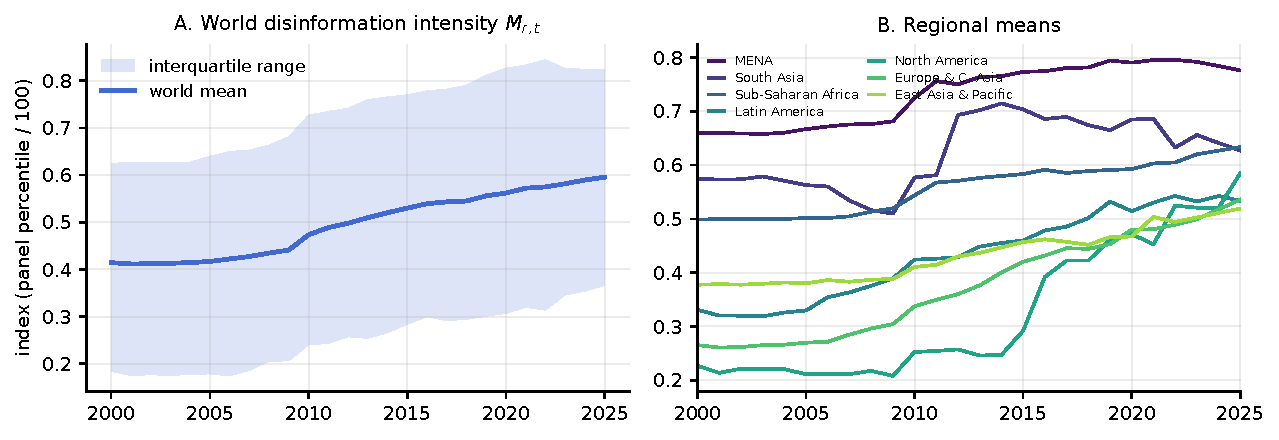
\includegraphics[width=\linewidth]{figures/fig1_index_trends.pdf}
\caption{The retrospective disinformation index. The world mean, interquartile
range and regional means describe relative positions in a pooled distribution,
not estimated shares of false financial messages.}\label{fig:index}
\end{figure}

\subsection{Outcomes and conditioning variables}\label{subsec:outcomes}
Real GDP, gross fixed capital formation and export growth are WDI annual
percentage changes \citep{worldbank2026wdi}. Capital formation is labeled
\emph{investment}; it does not specifically identify innovation finance.
Gini and nonperforming-loan (NPL) ratios provide distributional and banking
outcomes. These outcome series are never interpolated or filled in the
estimation. Growth outcomes sum observed annual rates from $t$ to $t+h$;
this is a cumulative percentage-point sum, not compounded GDP-level growth.
Gini and NPL outcomes are observed endpoint changes from $t-1$ to $t+h$.

Conditioning states are NPLs, trade openness and inequality. Missing NPL
conditioning values may use the previous observation for at most two years;
Gini conditioning values may use it for at most five years. No future
observation is used to fill these states, and a no-fill specification is
reported separately. The frozen input includes two-sided interpolated columns
for provenance; they are replaced in memory before estimation. Calendar-year
matching prevents a gap from being mistaken for a one-year lag.

Controls include lagged GDP growth, log real GDP per capita, CPI inflation
clipped to $[-10,60]$, and government effectiveness. Investment and export equations also
include the lagged observed outcome; lagged NPL and Gini levels already enter
as conditioning states. The frozen WGI vintage ends in 2022 and
its existing forward-carried values are retained through 2025; an end-2022
sample check is reported. Historical source releases and contemporaneous
publication dates are not reconstructed, so the forecasting exercise uses
latest-vintage data and cannot be described as real-time validation.

\input{tables/summary_table}

\section{Conditional Estimates and Predictive Validation}\label{sec:empirics}

\subsection{Estimation and interpretation}\label{subsec:estimation}
The latent-state regression is
\begin{equation}\label{eq:stateemp}
 x_{r,t+1}=\alpha_r+\lambda_t+\rho x_{r,t}+\delta s_{r,t}
 +\theta_1 F_{r,t}+\theta_2F_{r,t}x_{r,t}+\theta_3\pi_{r,t}+u_{r,t+1},
\end{equation}
where $s_{r,t}$ is the leave-one-out regional mean of the latent index.
Banking stress is standardized within country in this equation. Regional
co-movement is not necessarily transmission: regional economic or political
shocks can affect both the index and neighboring countries.

For outcome $k$ and horizon $h=0,\ldots,4$, the local projection is
\begin{equation}\label{eq:lp}
 Y^{(k)}_{r,t,h}=\alpha^{(k,h)}_r+\lambda^{(k,h)}_t+
 \beta^{(k)}_h M^z_{r,t}+\phi^{(k)\top}_h(M^z_{r,t}W_{r,t})
 +\eta^{(k)\top}_hW_{r,t}+\Gamma^{(k)\top}_h Z^{(k)}_{r,t}
 +e^{(k)}_{r,t,h}.
\end{equation}
$M^z$ is the standardized index and $W$ contains standardized NPLs, trade
openness and Gini measured at $t-1$. $Z$ contains clipped inflation, log GDP per capita,
government effectiveness, lagged growth and, for investment and exports, the
lagged observed outcome. Country and year effects are estimated by iterated
within transformation. Standard errors cluster by country. All leads and
lags refer to calendar years. For cumulative growth, $h=1$ is two years and
$h=2$ is three years, including the current observation at $t$.

The coefficient $\beta_h$ is the slope at mean conditioning states, not
necessarily the population-average marginal effect in the unbalanced
estimation sample. The plotted slope at stress $f$ is $\beta_h+\phi_{F,h}f$;
its variance includes $2f\operatorname{Cov}(\hat\beta_h,\hat\phi_{F,h})$.
Omitting this covariance is not generally conservative. Country clustering
allows within-country dependence but does not eliminate residual regional
dependence; a Driscoll--Kraay check is reported in the appendix. Leave-region-out estimates assess sensitivity to regional
composition; they are not a substitute for spatially robust inference.

\subsection{Index persistence}\label{subsec:persistence}
\begin{table}[!htbp]
\centering\small
\caption{Conditional index dynamics}\label{tab:state}
\begin{tabular}{lrr}\toprule
Regressor & Estimate & SE \\
\midrule
Index persistence & 0.864*** & (0.054) \\
Regional association & 0.184*** & (0.048) \\
Banking stress & 0.002 & (0.008) \\
Stress $\times$ latent index & -0.011* & (0.006) \\
Inflation & -0.044 & (0.040) \\
\bottomrule\end{tabular}
\par\smallskip\begin{minipage}{0.98\linewidth}\footnotesize Country and year effects; 2,090 observations from 135 countries. Stress is standardized within country. The persistence adjustment discussed in the text is an uncapped approximation.\end{minipage}
\end{table}

The revised state equation uses \StateN\ observations from
\StateCountries\ countries. Estimated persistence is $\Rho$ (SE $\RhoSE$),
with a scalar latent-index half-life of $\HalfLife$ years conditional on
other regressors. Applying the rough Nickell adjustment
$\hat\rho+(1+\hat\rho)/\bar T$ gives $\RhoBC$, without capping the result.
This approximation is not a validated correction for the full interacted,
unbalanced specification. An adjusted value at or above one has no finite
stationary half-life under Proposition~\ref{prop:state}. For comparison,
$\rho=0.99$ would imply about 69 years, not eight to nine.

The sum of the fitted baseline persistence and regional coefficient is
$\NetworkSlope$. In the simplified homogeneous endogenous-network model,
a sum above one fails the stability condition. The fitted equation includes
fixed effects and stress interactions, so this calculation is a diagnostic,
not a complete network estimate. It rules out treating the scalar estimate
alone as evidence that the whole regional system is stationary. Neither the
index half-life nor its bias adjustment identifies the duration of individual
false narratives.

\subsection{Mean associations and fragility interactions}\label{subsec:lp}
\input{tables/revised_lp}
The three-year growth slope at mean conditioning states is $\GrowthTwo$
percentage points, with a stress interaction of $\FragilityTwo$ points.
Table~\ref{tab:lp} reports uncertainty for every outcome and horizon. These
are conditional associations with a persistent index, rather than impulse
responses to an exogenous innovation. Contemporaneous macroeconomic controls
and lagged conditioning states may themselves respond to disinformation or common
shocks, which further prevents a total causal interpretation.

The investment, inequality and NPL estimates are supplementary evidence.
A fall in measured inequality is not an increase in inequality harm, an
insignificant estimate is not evidence of an exact zero, and average NPL
associations cannot establish a stress-feedback mechanism. Interpretation of
the financing hypothesis rests on the sign and uncertainty of the growth
interaction, its stability across specifications, and the limitations of NPLs
as a proxy for financing pressure. At $h=2$, the no-fill growth slope is
$-0.45$ (SE $0.74$), while its stress interaction remains negative
($-1.02$, SE $0.27$). In the post-2015 sample the interaction is $-0.10$
(SE $0.61$), and it is imprecise when Europe and Central Asia are omitted.
Thus the baseline evidence does not establish a stable contemporary effect
across every sample or conditioning choice.

\begin{figure}[!htbp]\centering
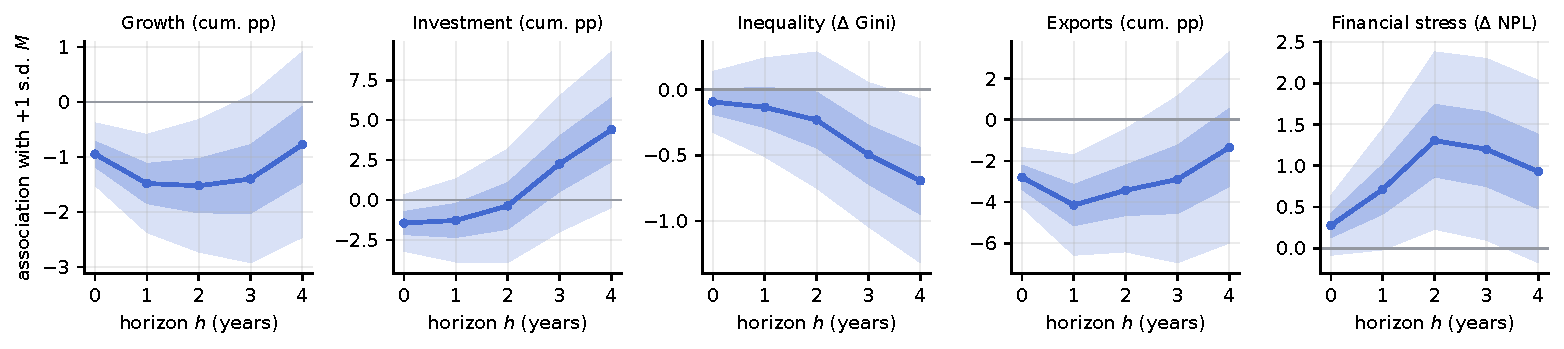
\includegraphics[width=\linewidth]{figures/fig2_lp_irfs.pdf}
\caption{Conditional mean slopes at mean conditioning states. Bands are
50 and 90 percent normal-approximation intervals from country-clustered
standard errors. Gini and NPL outcomes use observed endpoints.}\label{fig:lp}
\end{figure}
\begin{figure}[!htbp]\centering
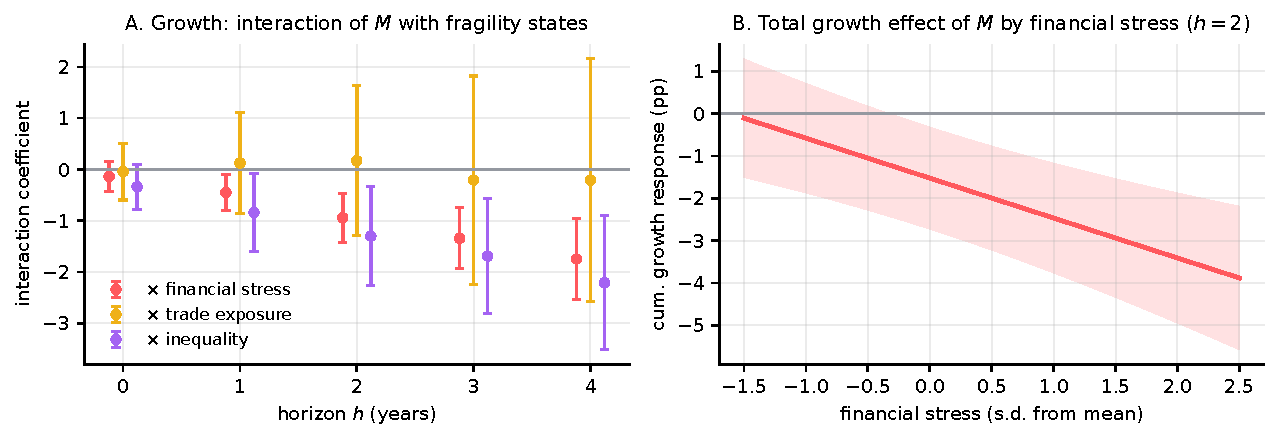
\includegraphics[width=\linewidth]{figures/fig3_amplification.pdf}
\caption{Growth interactions and the slope conditional on banking stress.
The right panel includes the estimated covariance between the index and its
stress interaction. Curves describe an estimated regression surface, not a
policy treatment response.}\label{fig:amplification}
\end{figure}

\subsection{Conditional quantiles and joint uncertainty}\label{subsec:gar}
For two-year cumulative growth, the first stage fits a two-way fixed-effects
mean regression on the index, NPLs, clipped inflation, lagged growth, log GDP
per capita and governance. Additive country and year effects are recovered
by backfitting and removed from the outcome. The second stage fits pooled
quantile regressions on the original covariates and an intercept, following
the location-shift logic of \citet{canay2011simple}. It is not quantile
regression of within-demeaned outcomes on within-demeaned regressors.

The assumption that country and year effects are common location shifts
across quantiles is substantive and cannot be justified merely because the
interest is in slopes. The procedure estimates a conditional distribution,
not the outcome that the same country would experience under a treatment.
Its covariate set is simpler than the mean-interaction specification; the
results are complementary rather than numerically identical estimands.

The revised implementation uses a linear-programming quantile solver and
\BootReps\ country-block bootstrap draws. Each draw resamples complete
country histories with replacement, assigns new identifiers to repeated
countries, and re-estimates both the mean-effect and quantile stages.
Ninety-percent percentile intervals and paired slope contrasts incorporate
the first-stage estimation step. They condition on the constructed index;
expert-coding uncertainty and residual cross-country dependence are not
fully included.
\input{tables/revised_quantiles}
\input{tables/revised_contrasts}
The point estimates at the tenth, median and ninetieth quantiles are
$\QuantileTen$, $\QuantileFifty$ and $\QuantileNinety$. Whether the lower-tail
slope is distinguishable from the center or upper tail is assessed directly
in Table~\ref{tab:contrasts}. The paired tests do not reject equal slopes (tenth versus median,
$p=0.575$; tenth versus ninetieth, $p=0.805$). All reported quantile
slope intervals include zero. The earlier claim of a statistically distinct,
roughly threefold lower-tail association is therefore withdrawn.
\begin{figure}[!htbp]\centering
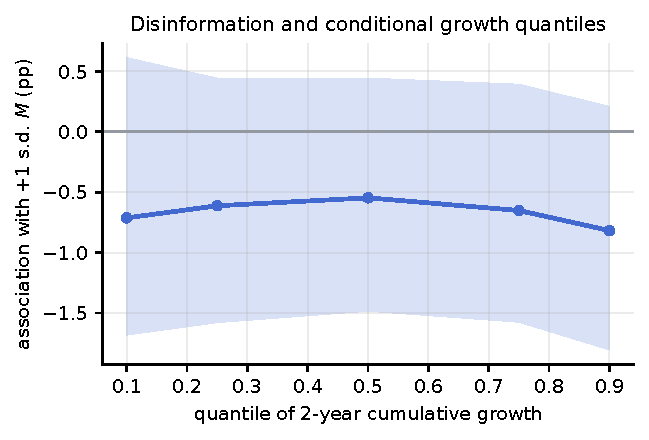
\includegraphics[width=.67\linewidth]{figures/fig4_growth_at_risk.pdf}
\caption{Conditional quantile slopes with 90 percent country-block bootstrap
intervals. Both estimation stages are refitted in each draw.}\label{fig:gar}
\end{figure}

\subsection{Reverse timing and identification limits}\label{subsec:identification}
Country and year effects remove additive persistent differences and common
year shocks. They do not remove time-varying institutional deterioration,
conflict, political instability or reverse causality. Associations with prior
outcomes are reported in Appendix~\ref{app:empirical}. Because the index is
persistent and lagged-outcome controls overlap the placebo windows, these
reverse-timing regressions are diagnostics, not experimental pre-trend tests.
In particular, controlling for a dependent variable's own overlapping lag
cannot establish the absence of confounding.

The previous draft's regional-pressure instrument interacted with internet
penetration does not establish identification. Internet exposure may affect
growth through other channels; regional pressure may reflect regional shocks;
and 2000--2004 exposure is not pre-period for a sample beginning in 2000.
Weak-IV estimates with large uncertainty cannot validate the sign. The
revised paper withdraws that evidence rather than treating it as causal
corroboration. The repository retains the original results in a clearly
marked legacy directory for audit, with the optional IV implementation
restricted to post-2004 observations and its excluded-instrument diagnostic
corrected. It is not part of the revised empirical evidence.

\subsection{Chronological forecast evaluation}\label{subsec:forecast}
At each annual origin $t=2014,\ldots,2023$, the exercise predicts GDP growth
in $t+1$ using covariates from $t-1$. Training targets end no later than
$t-1$. This conservative timing prevents use of current-year realized growth
or a future outcome in model fitting. Each model uses the same observed
sample and country intercepts; no future year effect is estimated.

The benchmark contains growth, clipped inflation, log GDP per capita, trade
openness, NPLs, private credit and government effectiveness. Missing NPL and
credit predictors can be carried forward for at most two years, never
backward. The augmented model adds the DSP index. All five component
standardizations, the rank transform, and regression scaling are fitted anew
using training observations only. Models estimate the conditional mean and
the tenth, median and ninetieth quantiles directly. The benchmark and augmented
models use identical training and evaluation samples at each origin.

\input{tables/revised_forecast}
The tenth-quantile loss gain is $\ForecastTail$ percent and the mean-squared
error gain is $\ForecastMean$ percent. Negative gains denote deterioration. None of the four loss metrics
improves at the point estimate; the tenth-quantile gain interval includes
zero. These results do not establish operational forecasting value for this
index and benchmark. Country-specific intercepts with sparse training
histories and omitted common-shock predictors may also limit performance.
Intervals resample complete target years, preserving dependence among
countries in a given year, but ten target years provide limited precision
and do not fully address serial dependence across years. The exercise is
pseudo out of sample: source vintages may contain revisions, expert scores
may be retrospective, and their actual publication calendars are not
reconstructed. A useful association in the panel therefore need not imply
an operational early-warning improvement.

\section{What Can Be Quantified as Risk?}\label{sec:risk}

The defensible quantitative outputs are conditional growth profiles,
uncertainty intervals, observed banking-stress interactions, and held-out
forecast losses. At an observed stress value $f$, the reported profile is
$\hat\beta_h+\hat\phi_{F,h}f$, with other conditioning states at their
reference values. It should be evaluated within the empirical support and
with its covariance-based uncertainty. A change in this profile is not an
estimated intervention effect.

The earlier twelve-year growth scenarios are withdrawn. The original code
convolved cumulative local-projection coefficients with repeated deviations
in the index level and divided the result by $\sqrt{H}$. Neither overlapping
cumulative coefficients nor this scaling identifies annual growth responses
to a sequence of structural shocks. Differencing cumulative coefficients
alone would not repair the additional problem that the regressor is a
persistent, endogenous level rather than an identified innovation.
A replacement scenario system would require explicit dynamic equations,
shock identification, and validation of the mapping from interventions to
parameters. Those ingredients are not supplied by the current panel.

The composite burden score is also withdrawn from quantitative claims.
Normalizing a channel by its estimated two-year response is unstable when
that response is near zero and uncertain. Reversals of the previous
stability-only ranking cannot be dismissed as an uninformative case while
claiming a general ordering. A bounded mathematical score does not establish
welfare meaning, comparability, or reliable policy rankings. The appendix
retains the elementary boundedness result solely to document the mathematical
scope of the original construction. No GDP-loss totals, burden reductions,
or empirical trap thresholds are inferred from it.

\section{Policy Interpretation and Research Requirements}\label{sec:policy}

The results motivate scrutiny of the information environment alongside
financial fragility, subject to the predictive validation in
Table~\ref{tab:forecast}. They do not establish that collecting the proposed
index improves decisions, that a financial rumor persists for the aggregate
index's half-life, or that a measured country is near a crisis threshold.

Rapid official communication, message authentication and restrictions on
content propagation are distinct candidate interventions. Their effects may
span the model intercept, persistence, innovation variance, public trust and
the reach of accurate information. Ranking them requires estimates of these
responses, implementation costs and possible adverse effects. The conditional
elasticity result in Proposition~\ref{prop:burden} does not provide those
estimates. Equation~\eqref{eq:cost} makes the missing comparison explicit.

A stronger policy study would link independently identified financial
falsehoods to audience exposure, bank funding or lending outcomes and
credible correction timings. It would then estimate the response to an
intervention using a design with a defensible counterfactual, rather than
relabeling a country-level association. A financial-content validation sample
would also test whether the broad DSP proxy captures the mechanism proposed
here. Out-of-time and real-time validation against richer financial-condition,
uncertainty and geopolitical-risk benchmarks would be needed before proposing
an operational monitoring instrument. These are requirements for stronger
claims, not results claimed by the present paper.

\section{Conclusion}\label{sec:conclusion}

A broad disinformation index can be examined as a correlate of macroeconomic
risk without equating political-information scores with financial-message
contamination. The panel estimates a three-year cumulative-growth
slope of $\GrowthTwo$ percentage points at mean conditioning states and a
banking-stress interaction of $\FragilityTwo$. Quantile inference and
chronological prediction evaluate the scope of the evidence, including the
possibility that in-sample associations do not improve held-out forecasts.

The illustrative financing model supplies an increasing-differences result
under an explicitly assumed lending rule. Feedback can generate multiple
steady states for some parameters, but the empirical exercise does not
identify a trap threshold. Persistence comparative statics rank parameter
changes only under sign and effectiveness restrictions; they do not identify
policy cost-effectiveness. The remaining contribution is a reproducible
conditional analysis, with measurement, identification and forecasting
limitations made explicit. Financial-specific data and credible intervention
variation are the next steps needed to support causal policy conclusions.


\clearpage
\begingroup\small
\bibliographystyle{plainnat}
\bibliography{bib/refs}
\endgroup

\clearpage
\appendix
\section{Proofs and Formalization Scope}\label{app:proofs}

\subsection{Scalar state dynamics}
The fixed-point equation $x=c+\rho x$ gives $\mu=c/(1-\rho)$.
Subtracting it from the recursion yields $x_{t+1}-\mu=\rho(x_t-\mu)$,
which proves the closed form and convergence for $|\rho|<1$.
Logistic bounds and strict monotonicity follow from $e^{-x}>0$.
With independent innovations, the stationary representation is
$x_t=\mu+\sum_{j\ge0}\rho^ju_{t-j}$ and the variance follows by a geometric
sum. Solving $\rho^h=1/2$ gives the latent half-life formula. These statements
condition on absent or fixed external inputs; they are not a stationarity
proof for the fitted regional panel.

For fixed nonnegative row-stochastic $W$, the vector of ones is an eigenvector
with eigenvalue one. Hence $\rho+\delta$ is an eigenvalue of
$A=\rho I+\delta W$. The induced infinity norm is $\rho+\delta$, so the
spectral radius is exactly that value for nonnegative $\rho,\delta$.
A time-varying network or country-dependent interaction coefficients require
a separate stability analysis.

\subsection{Signal noise and the lending assumption}
Independence gives $\E[b\eta]=0$ and
$\mathrm{Var}(b\eta d)=d^2\E[b\eta^2]=pd^2$. Adding independent
$\varepsilon$ proves Lemma~\ref{lem:pollution}. The posterior distribution
of $V$ has not been specified; the lemma does not compute its variance.
Under the assumed credit rule~\eqref{eq:credit},
\[
 I^*-\min\{I^*,W_0+L(p)\}
 =\max\{\lambda\gamma d^2p+I^*-W_0-\lambda\bar V
                   +\lambda\gamma\sigma_\varepsilon^2,0\}.
\]
Collecting the financing-pressure terms gives~\eqref{eq:harm}. This is a
conditional derivation from a stated reduced-form lending rule, not a
Bayesian microfoundation.

\subsection{Increasing differences}
Let $g(z)=\max\{z,0\}$, $s=ap_1+bF_1-\kappa_0$,
$u=a(p_2-p_1)\ge0$ and $v=b(F_2-F_1)\ge0$.
The increment $g(s+u)-g(s)$ is nondecreasing in $s$, which implies
$g(s+u)-g(s)\le g(s+v+u)-g(s+v)$. This proves increasing differences.
When $ap_2+bF-\kappa_0\le0$, both terms of the contamination increment
are zero. No quantitative claim about mean or quantile growth effects follows
without further assumptions on aggregation and other shocks.

\subsection{Feedback and multiplicity}
The map in~\eqref{eq:feedback} is globally Lipschitz with constant at most
$\rho+\varphi L_g$. When this bound is below one, Banach's fixed-point
theorem on the complete space $\R$ gives existence, uniqueness and global
convergence. In the piecewise-linear example, solving on each of
$x\le0$, $0\le x\le1$ and $x\ge1$ gives respectively $-3/2$, $1/2$ and
$5/2$. Slopes at those roots are $1/2$, $5/2$ and $1/2$.
The example proves that multiplicity is possible, not that it begins when
an upper bound on a derivative reaches one.

\subsection{Elasticities and the optional burden bound}
For $c>0$ and $0<\rho<1$,
\[
 \frac{\partial\mu}{\partial c}=\frac1{1-\rho},\qquad
 \frac{\partial\mu}{\partial\rho}=\frac{c}{(1-\rho)^2},\qquad
 \frac{\partial^2\mu}{\partial\rho^2}=\frac{2c}{(1-\rho)^3}.
\]
Multiplying the first derivatives by $c/\mu$ and $\rho/\mu$ establishes
Proposition~\ref{prop:burden}. The same algebraic elasticity identity extends
to $c\ne0$, but negative $c$ reverses the desired direction of a reduction
in persistence. At $c=0$, division by $\mu$ is undefined. Applying the chain
rule to expenditure gives~\eqref{eq:cost}.

For completeness, if $M_h\in[0,1]$, $|Y_h|\le\bar Y$ and $\kappa>0$,
then $D_H=\sum_{h=0}^H(1+\kappa)^{-h}M_hY_h$ satisfies
$|D_H|\le\bar Y(1+\kappa)/\kappa$ by the triangle inequality and the
geometric-series bound. Signed outcomes permit negative scores. This bound
is not a welfare result and does not validate the withdrawn normalization.

\subsection{What the Lean files establish}
The repository includes proofs of logistic bounds and monotonicity;
scalar deterministic dynamics and a geometric variance identity;
increasing differences of the max-linear harm function; uniqueness given a
contraction bound and an explicit three-root example; an absolute burden
bound; and algebraic derivative, elasticity and midpoint-convexity results.
These are selected mathematical statements, not a machine verification of
all economic interpretations. In particular, the files do not establish
construct validity, posterior-risk microfoundations, empirical identification,
forecast performance, intervention effectiveness, stochastic ergodicity of
the full panel, or a data-calibrated bifurcation threshold. The formalization
mapping and build instructions are recorded in the repository.

\section{Additional Empirical Evidence}\label{app:empirical}
\input{tables/revised_placebo}
\begin{table}[!htbp]
\centering\small
\caption{Growth associations under alternative specifications ($h=2$)}\label{tab:robustness}
\begin{tabular}{lrrrr}\toprule
Specification & $M$ & SE & $M\times F$ & $n$ \\
\midrule
dk & -1.52*** & (0.39) & -0.94** & 1,539 \\
domestic\_only & -1.56** & (0.70) & -0.88*** & 1,539 \\
end2022 & -0.78 & (0.84) & -0.72** & 1,232 \\
equal\_weights & -1.43* & (0.75) & -0.99*** & 1,539 \\
index\_history & -2.44*** & (0.77) & -0.96*** & 1,539 \\
no\_fill & -0.45 & (0.74) & -1.02*** & 1,041 \\
Omit East Asia \& Pacific & -1.57** & (0.78) & -1.05*** & 1,361 \\
Omit Europe \& Central Asia & -1.69 & (1.20) & -0.90 & 879 \\
Omit Latin America \& Caribbean & -2.28*** & (0.79) & -0.93*** & 1,297 \\
Omit Middle East \& North Africa & -1.68** & (0.72) & -1.00*** & 1,447 \\
Omit North America & -1.63** & (0.75) & -0.92*** & 1,507 \\
Omit South Asia & -1.27* & (0.72) & -0.91*** & 1,484 \\
Omit Sub-Saharan Africa & -0.67 & (0.77) & -0.85*** & 1,259 \\
post2015 & -1.51* & (0.81) & -0.10 & 839 \\
raw\_composite & -1.45* & (0.83) & -0.94*** & 1,539 \\
\bottomrule\end{tabular}
\par\smallskip\begin{minipage}{0.98\linewidth}\footnotesize No-fill uses observed conditioning states only. Raw-composite uses the unranked weighted index; each index is standardized in its specification. Alternative weights and samples can change results; stability is not presumed.\end{minipage}
\end{table}


Alternative-weight specifications reconstruct the index from the published
components. The raw-composite check removes the empirical-CDF transformation.
Sample restrictions, no-fill conditioning, a lagged-index control,
Driscoll--Kraay inference and leave-region-out estimates are explicitly
recomputed. Their signs, uncertainty and sample sizes should be compared with
the baseline rather than summarized as uniformly robust. The
Driscoll--Kraay calculation applies a Bartlett kernel with bandwidth two to
year-aggregated within-regression scores; inference uses year-count minus one
degrees of freedom. The short time dimension limits this approximation.
A lagged-index specification asks whether the current index adds information
conditional on its recent history, which is a different estimand from the
baseline level association.

The Monte Carlo exercise simulates the repository's own stylized
linear-interaction data-generating process in 200 replications. Its output
is retained as a numerical estimator diagnostic. It does not test the DSP
measurement process, time-varying confounding, the revised forecasting
exercise or the assumed financing mechanism. Bias correction reduces but
need not eliminate dynamic-panel bias.

\section{Replication and Data Provenance}\label{app:replication}
The public repository is
\url{https://github.com/jameskrice7/Financial-Disinformation-as-a-Macroeconomic-Risk}.
The revised source, figures and tables are versioned with the empirical code.
The entry point \texttt{code/scripts/run\_all.py} uses the frozen merged
panel and a separately documented extraction of DSP v8 components.
It regenerates state and local-projection estimates, all reported robustness
checks, quantile bootstrap draws and contrasts, held-out predictions and
losses, Monte Carlo diagnostics, figures, table environments and numerical
macros used in the text. Source hashes and software versions accompany the
outputs. The main analysis runs without downloading a new WDI vintage.

The frozen panel contains observed and historically interpolated columns.
The revised pipeline preserves observed outcomes, replaces conditioning
columns with limited forward carries, and fits forecasting transformations
within training windows. Data coverage is not identical to complete-case
regression coverage. A separate provenance record identifies source URLs,
retrieval information available for this revision, and the limitations of the
older merged panel. Its original raw-vintage details cannot be reconstructed
from an undocumented download date, so the paper makes no real-time claim.

Legacy scenario, IV and burden outputs are retained only for audit under
\texttt{output/legacy}. They do not feed the revised paper. Numerical tests
cover calendar alignment, observed outcomes, training-only transformations,
bootstrap contrasts and covariance propagation. Source changes and remaining
research limitations are documented in the revision note.


\end{document}
